\documentclass[xetex,mathserif,serif]{beamer}

\usepackage{xunicode}
\usepackage{xltxtra}
\usepackage{color}
\usepackage{url}
\usepackage{listings}
\usepackage{fontspec}
\usepackage{geometry}
\usepackage{lastpage}
\usepackage{fancyhdr}
\usepackage{amsmath}
\usepackage{amsthm}
\usepackage{amssymb}
\usepackage{blkarray}
\usepackage{multicol}
\usepackage{relsize}

\definecolor{solarized@base03}{HTML}{002B36}
\definecolor{solarized@base02}{HTML}{073642}
\definecolor{solarized@base01}{HTML}{586e75}
\definecolor{solarized@base00}{HTML}{657b83}
\definecolor{solarized@base0}{HTML}{839496}
\definecolor{solarized@base1}{HTML}{93a1a1}
\definecolor{solarized@base2}{HTML}{EEE8D5}
\definecolor{solarized@base3}{HTML}{FDF6E3}
\definecolor{solarized@yellow}{HTML}{B58900}
\definecolor{solarized@orange}{HTML}{CB4B16}
\definecolor{solarized@red}{HTML}{DC322F}
\definecolor{solarized@magenta}{HTML}{D33682}
\definecolor{solarized@violet}{HTML}{6C71C4}
\definecolor{solarized@blue}{HTML}{268BD2}
\definecolor{solarized@cyan}{HTML}{2AA198}
\definecolor{solarized@green}{HTML}{859900}
\definecolor{yaleblue}{HTML}{0E4C92}

\setbeamertemplate{navigation symbols}{}
% \setbeamerfont{title}{family=\old}
% \setbeamerfont{author}{family=\tfont}%
% \setbeamerfont{frametitle}{family=\oldA}
% \setbeamerfont{date}{family=\dfont}

\setbeamertemplate{itemize items}{--}
\setbeamercolor*{item}{fg=black}

\defaultfontfeatures{Mapping=tex-text}
\hypersetup{pdfstartview={FitH}}

\newcommand{\old}[1]{\fontspec[Alternate=1,Ligatures={Common}]{Hoefler Text}\fontsize{18pt}{30pt}\selectfont #1}%
\newcommand{\oldA}[1]{\fontspec[Alternate=1,Ligatures={Common, Rare}]{Hoefler Text}\fontsize{12pt}{15pt}\selectfont #1}%
\newcommand{\oldB}[1]{\fontspec[Ligatures={Common}]{Didot}\fontsize{12pt}{15pt}\color{solarized@base02}\selectfont #1}%
\newcommand{\tfont}[1]{\fontspec[Alternate=1,Ligatures={Common}]{Hoefler Text}\fontsize{12pt}{20pt}\selectfont #1}%
\newcommand{\dfont}[1]{\fontspec[Ligatures={Common}]{Didot}\fontsize{12pt}{12pt}\selectfont #1}%

\newcommand{\minimize}{\mathop{\mathrm{minimize}}}
\newcommand{\argmin}{\mathop{\mathrm{arg\,min}}}
\newcommand{\argmax}{\mathop{\mathrm{arg\,max}}}
\newcommand{\st}{\mathop{\mathrm{subject\,\,to}}}

\newcommand\independent{\protect\mathpalette{\protect\independenT}{\perp}}
\def\independenT#1#2{\mathrel{\rlap{$#1#2$}\mkern2mu{#1#2}}}

\setlength{\parindent}{0pt}
\setlength{\parskip}{12pt}

\setromanfont [Ligatures={Common}, Numbers={OldStyle}, Variant=01,
 BoldFont={LinLibertine_RB.otf},
 ItalicFont={LinLibertine_RI.otf},
 BoldItalicFont={LinLibertine_RBI.otf}
 ]{LinLibertine_R.otf}



\begin{document}

%%%%%%%%%%%%%%%%%%%%%%%%%%%%%%%%%%%%%%%%%%%%%%%%%%%
\begin{frame}[fragile] \frametitle{}

\vfill

{\fontsize{0.7cm}{0cm}\selectfont Lecture 05 \\\vspace{0.2cm}
Geometry of Least Squares}\\\vspace{0.5cm}
16 September 2015

\vspace{2cm}

\begin{minipage}{0.6\textwidth}
Taylor B. Arnold \\
Yale Statistics \\
STAT 312/612
\end{minipage}
\hfill
\begin{minipage}{0.3\textwidth}\raggedleft

\includegraphics[scale=0.3]{../yale-logo.png}
\end{minipage}%

\end{frame}

%%%%%%%%%%%%%%%%%%%%%%%%%%%%%%%%%%%%%%%%%%%%%%%%%%%
\begin{frame}[fragile] \frametitle{}

{\color{yaleblue}\fontsize{16pt}{20pt}\selectfont Goals for today}

\begin{enumerate}
\item Geometry of least squares
\item Projection matrix P and annihilator matrix M
\item Multivariate Galton Heights
\end{enumerate}

\end{frame}

%%%%%%%%%%%%%%%%%%%%%%%%%%%%%%%%%%%%%%%%%%%%%%%%%%%
\begin{frame}[fragile] \frametitle{}

\begin{flushright}
{\color{yaleblue}\sc\fontsize{1cm}{0cm}\selectfont Geometry of Least Squares}
\end{flushright}

\end{frame}

%%%%%%%%%%%%%%%%%%%%%%%%%%%%%%%%%%%%%%%%%%%%%%%%%%%
\begin{frame}[fragile] \frametitle{}

Last time, we established that the least squares solution to the
model:
\begin{align*}
y &= X\beta + \epsilon
\end{align*}
Yields the solution:
\begin{align*}
\widehat{\beta} &= (X^t X)^{-1} X^t y
\end{align*}
As long as the matrix $X^t X$ is invertable.

\end{frame}

%%%%%%%%%%%%%%%%%%%%%%%%%%%%%%%%%%%%%%%%%%%%%%%%%%%
\begin{frame}[fragile] \frametitle{}

Define the column space of the matrix $X$ as:
\begin{align*}
\mathcal{R} (X) &= \left\{ \theta : \theta = X b, \, b \in \mathbb{R}^p \right\} \subset \mathbb{R}^n
\end{align*}
This is the space spanned by the $p$ columns of $X$ sitting in $n$-dimensional space.

\pause Notice that the least squares problem can be re-written as:
\begin{align*}
\widehat{\theta} &= \argmin_\theta \left\{ || y - \theta||_2^2, \quad \text{s.t} \quad \theta \in \mathcal{R} (X) \right\}
\end{align*}
Where then $\widehat{\beta} = X \widehat{\theta}$.

\end{frame}

%%%%%%%%%%%%%%%%%%%%%%%%%%%%%%%%%%%%%%%%%%%%%%%%%%%
\begin{frame}[fragile] \frametitle{}

{\bf Theorem 3.2 (p.g. 37, Rao \& Toutenburg)} The minimum, $\widehat{\theta}$ is
attained when $(y - \widehat{\theta}) \perp \mathcal{R}(X)$.
In other words, $(y - \widehat{\theta})$ is perpendicular to all vectors
in $\mathcal{R}$.

\end{frame}

%%%%%%%%%%%%%%%%%%%%%%%%%%%%%%%%%%%%%%%%%%%%%%%%%%%
\begin{frame}[fragile] \frametitle{}

{\it Proof}: Pick a $\widehat{\theta}$ in $\mathcal{R}$ such that
$(y - \widehat{\theta}) \perp \mathcal{R}(X)$. \pause This implies
that $X^{t} (y - \widehat{\theta}) = 0$. Then for all $\theta \in \mathcal{R}$:
\begin{eqnarray*}
|| y - \theta ||_2^2 &=& (y - \widehat{\theta} + \widehat{\theta} - \theta)^t (y - \widehat{\theta} + \widehat{\theta} - \theta) \\ \pause
&=& (y - \widehat{\theta})^t (y - \widehat{\theta}) + (\widehat{\theta} - \theta)^t (\widehat{\theta} - \theta) +
    2 (y - \widehat{\theta})^t (\widehat{\theta} - \theta) \\ \pause
&=& (y - \widehat{\theta})^t (y - \widehat{\theta}) +
    (\widehat{\theta} - \theta)^t (\widehat{\theta} - \theta) \\ \pause
&=& || y - \widehat{\theta} ||^2_2 + || \widehat{\theta} - \theta ||_2^2 \\ \pause
&\geq& || y - \widehat{\theta} ||^2_2 \pause
\end{eqnarray*}
So, if such a $\widehat{\theta}$ exists it attains the minimum. To see that
it does, write $\widehat{\theta} = X \widehat{\beta}$. \pause Then:
\begin{eqnarray*}
X^t ( y - \widehat{\theta} ) &= X^t ( y - X \widehat{\beta} ) \\
&= X^t y - X^t X \widehat{\beta}
\end{eqnarray*}

\end{frame}

%%%%%%%%%%%%%%%%%%%%%%%%%%%%%%%%%%%%%%%%%%%%%%%%%%%
\begin{frame}[fragile] \frametitle{}

To see that such a $\widehat{\theta}$ does exist,
write $\widehat{\theta} = X \widehat{\beta}$. \pause Then:
\begin{eqnarray*}
X^t ( y - \widehat{\theta} ) &=& X^t ( y - X \widehat{\beta} ) \\ \pause
&=& X^t y - X^t X \widehat{\beta} \\ \pause
&=& X^t y - X^t X (X^t X)^{-1} X^t y \\ \pause
&=& X^t y - X^t y \\
&=& 0
\end{eqnarray*}
And therefore our proposed $\widehat{\theta} \in \mathcal{R}(X)$.

\end{frame}

%%%%%%%%%%%%%%%%%%%%%%%%%%%%%%%%%%%%%%%%%%%%%%%%%%%
\begin{frame}[fragile] \frametitle{}

From this geometric interpretation of the least squares estimator,
we introduce an important matrix $P_X$ called the {\it projection matrix}.
\begin{align*}
P_X &= X (X^t X)^{-1} X^t
\end{align*}
I'll often drop the subscript as it should be understood that the
projection is on the data matrix $X$.

\end{frame}

%%%%%%%%%%%%%%%%%%%%%%%%%%%%%%%%%%%%%%%%%%%%%%%%%%%
\begin{frame}[fragile] \frametitle{}

Notice that $PX=X$:
\begin{align*}
P X &= X (X^t X)^{-1} X^t X \\
&= X
\end{align*}
\pause And $Py$ gives the fitted values $\widehat{y}$:
\begin{align*}
P y &= X (X^t X)^{-1} X^t X y \\
&= X \widehat{\beta} \\
&= \widehat{\theta} \\
&= \widehat{y}
\end{align*}
Do you see why the projection matrix is called the projection
matrix? \pause

\end{frame}

%%%%%%%%%%%%%%%%%%%%%%%%%%%%%%%%%%%%%%%%%%%%%%%%%%%
\begin{frame}[fragile] \frametitle{}

\begin{center}
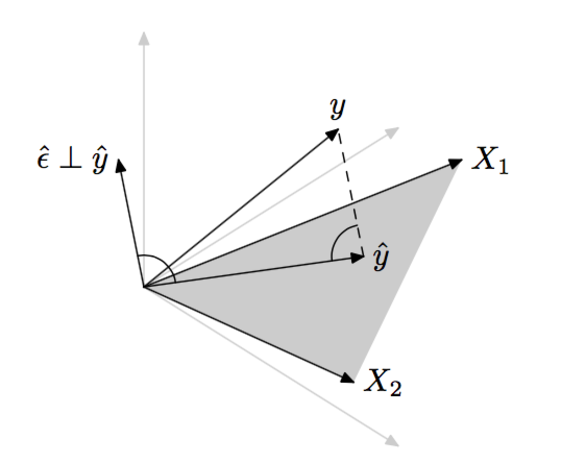
\includegraphics[width=4in]{img/olsGeom.pdf}
\end{center}

\end{frame}

%%%%%%%%%%%%%%%%%%%%%%%%%%%%%%%%%%%%%%%%%%%%%%%%%%%
\begin{frame}[fragile] \frametitle{}

The projection matrix is sometimes called the {\it hat matrix}.
Any thoughts as to why?

\end{frame}

%%%%%%%%%%%%%%%%%%%%%%%%%%%%%%%%%%%%%%%%%%%%%%%%%%%
\begin{frame}[fragile] \frametitle{}

A closely related matrix to $P$ is the {\it annihilator matrix}
$M$:
\begin{align*}
M = I_n - P
\end{align*}
\pause It gets its name because $MX = 0$.

\end{frame}

%%%%%%%%%%%%%%%%%%%%%%%%%%%%%%%%%%%%%%%%%%%%%%%%%%%
\begin{frame}[fragile] \frametitle{}

The matrix $P = X (X^t X)^{-1} X^t$ is clearly symmetric.
It is also idempotent:
\begin{eqnarray*}
P^2 &=& {\color{solarized@magenta} X (X^t X)^{-1} X^t}  {\color{solarized@blue} X (X^t X)^{-1} X^t}\\ \pause
&=& X {\color{solarized@red} (X^t X)^{-1}} {\color{solarized@green} (X^t X)} {\color{solarized@red}(X^t X)^{-1}} X^t \\  \pause
&=& X (X^t X)^{-1} X^t \\  \pause
&=& P
\end{eqnarray*}

\end{frame}

%%%%%%%%%%%%%%%%%%%%%%%%%%%%%%%%%%%%%%%%%%%%%%%%%%%
\begin{frame}[fragile] \frametitle{}

M is also symmetric
\begin{align*}
M^t &= (I_n - P)^t \\
&= (I_n - P^t) \\
&= M
\end{align*}
\pause And idempotent:
\begin{eqnarray*}
M^2 &=&(I_n - P)^2 \\
&=& (I_n - P) (I_n - P) \\ \pause
&=& I_n - 2 * P + P^2 \\ \pause
&=& I_n - 2 * P + P \\ \pause
&=& I_n - P \\
&=& M
\end{eqnarray*}
\pause These properties both make sense given the geometric
interpretation of $P$ and $M$ as projections; into the column
space of $X$ and the compliment of the columns space of $X$.

\end{frame}

%%%%%%%%%%%%%%%%%%%%%%%%%%%%%%%%%%%%%%%%%%%%%%%%%%%
\begin{frame}[fragile] \frametitle{}

These properties are quite useful. Notice how we can
easily rewrite the following for the residual vector
$r = y - X\widehat{\beta}$:
\begin{eqnarray*}
r  &=& y - X\widehat{\beta} \\ \pause
&=& y - Py \\ \pause
&=& (I_n - P) y \\ \pause
&=& M y \\ \pause
&=& M (X \beta + \epsilon) \\ \pause
&=& M \epsilon \\
\end{eqnarray*}
\pause The matricies $P$ and $M$ not only help make the
derivation easier, they also give geometric insight into
what we are doing.

\end{frame}

%%%%%%%%%%%%%%%%%%%%%%%%%%%%%%%%%%%%%%%%%%%%%%%%%%%
\begin{frame}[fragile] \frametitle{}

One particularly useful formula will be writing the
squared residuals as:
\begin{align*}
||r||_2^2 &= || M \epsilon ||_2^2 \\
&= \epsilon^t M^t M \epsilon \\
&= \epsilon^t M \epsilon
\end{align*}
\pause So the matrix $M$ translates the sum of squared residuals
into the sum of the square errors, which are estimated by the
residuals.

\end{frame}

%%%%%%%%%%%%%%%%%%%%%%%%%%%%%%%%%%%%%%%%%%%%%%%%%%%
\begin{frame}[fragile] \frametitle{}

\begin{flushright}
{\color{yaleblue}\sc\fontsize{1cm}{0cm}\selectfont Applications}
\end{flushright}

\end{frame}


\end{document}











